\documentclass[11pt,a4 paper]{article}
\usepackage{amsmath, amsthm} 
\usepackage[english]{babel}
\usepackage[T1]{fontenc}
\usepackage[utf8]{inputenc}
\usepackage[margin=2cm]{geometry}
\usepackage{graphicx}
\usepackage{subfigure}
\usepackage{caption}
\usepackage{siunitx}
\captionsetup{tableposition=top,font=small,width=0.8\textwidth}
\usepackage{booktabs}
\usepackage[table]{xcolor}
\usepackage[arrowdel]{physics}
\usepackage{mathtools}
\usepackage{tablefootnote}
\usepackage{amssymb}
\usepackage{enumitem}
\usepackage{multicol}
\setlist[description]{font={\scshape}} %style=unboxed,style=nextline
\usepackage{wrapfig}
\usepackage{float}
\usepackage{floatflt}
\usepackage{url}
\usepackage{commath}
\usepackage{bm}
\usepackage[version=4]{mhchem}
\usepackage{nicefrac}
\usepackage{ifthen}
\usepackage{comment}
\usepackage[colorinlistoftodos,textsize=tiny]{todonotes}
\usepackage{hyperref}

\renewcommand*{\thefootnote}{\fnsymbol{footnote}}
\sisetup{exponent-product = \cdot}
\newcommand{\tc}{\,\mbox{tc}\,}
\newcommand{\Epsilon}{\mathcal{E}}
\newcommand{\half}{\frac{1}{2}}
\newcommand{\overbar}[1]{\mkern 1.5mu\overline{\mkern-1.5mu#1\mkern-1.5mu}\mkern 1.5mu}
\let\oldfrac\frac
\renewcommand{\frac}[3][d]{\ifthenelse{\equal{#1}{d}}{\oldfrac{#2}{#3}}{\nicefrac{#2}{#3}}}

\title{Positronium}
\author{Andrea Grossutti, mat. 1237344\\Alessandro Lovo, mat. 1236048\\Leonardo Zampieri, mat. 1237351}
\date{\today}

\begin{document}

\maketitle

\section{Aims}
\begin{itemize}
    \item Measure the ratio between the two and three photons decay of the Positronium;
    \item Measure the lifetime of the Positronium through the time distribution of the decays.
\end{itemize}

\section{Experimental setup}
The experimental setup consist in 4 inorganic scintillators; three coplanar (DET. 1,2,3) and a fourth (DET. 4) perpendicular to the plane.

The first three detector are placed on a circumference in the center of which lies a \ce{^22Na} source, with an activity of around $380\si{kBq}$. These detector are free movable around the circumference; in this session, two different configurations have been explored. To observe the two-photons decay, the detectors \#1 and \#2 have been aligned; instead, to observe the three-photons decay, the three coplanar detectors have been positioned to form an equilateral triangle.

Data are collected from the detectors through a electronic chain: a fan-in-fan-out quad module reply the signal of each detectors and produce four copies of it; then, through a CFD, a trigger signal is produced.  The CFD trigger threshold has been set so that the background noise is discarded, while the interesting signals produce an output. As can be seen from fig. \ref{fig:oscilloscope}, the signals corresponding to the detection of the $511\si{\kilo\electronvolt}$ and $1275\si{\kilo\electronvolt}$ photons are clearly visible.

\begin{figure}[H]
    \centering
    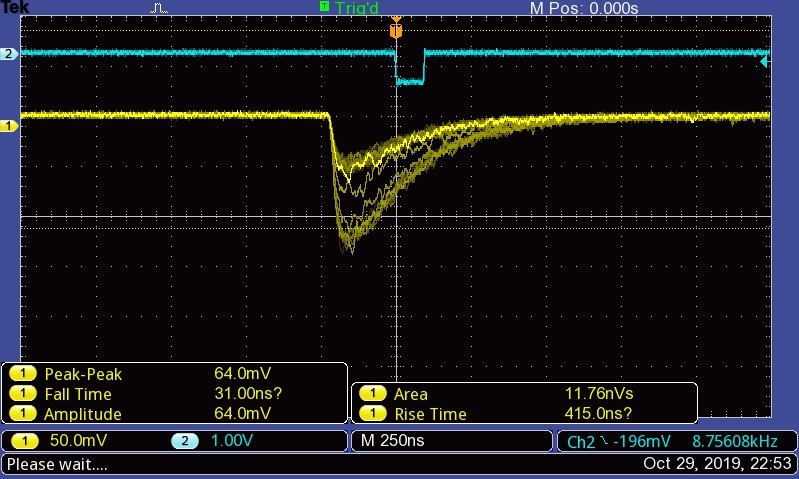
\includegraphics[width=0.7\textwidth]{img/TEK0001.JPG}
    \caption{Signal from the detector (yellow), triggering through the CFD (blu). The two different types of peaks, respectively for the $511\si{\kilo\electronvolt}$ and $1275\si{\kilo\electronvolt}$ photons, are clearly visible. Det. \#2.}
    \label{fig:oscilloscope}
\end{figure}

Between the second and the third day, a technical problem required the substitution of the high voltage power supply; due to this, thresholds have been re-set; moreover, in the middle of the day 3 the high voltage power supply burned; it has been replaced and the threshold re-set. While in the first two days all the detectors saw the two peaks around an amplitude of respectively $100$ and $250\si{\milli\volt}$ (and therefore the threshold has been set at about $75\si{\milli\volt}$), in the third day the detectors \#1 and \#3 saw the two peaks around an amplitude of respectively $50$ and $125\si{\milli\volt}$ (and therefore the threshold has been set at about $35\si{\milli\volt}$). For the detector \#4, finally, the threshold has been set to about $200\si{\milli\volt}$, such that only the higher energetic photons produce a trigger.

The CFT is provided of two sets of microswitches, to adjust delay and switch of the output signal. As has been verified thanks to the oscilloscope, the delay microswitches allow to adjust the time between the triggering of the system and the start of the logic signal, while the switch microswitches can be used to adjust the time length of the logic signal.

\section{Apparatus calibration}
Due to the various problem, the apparatus calibration has been done many times; only the first calibration is here reported, having for the other followed the same procedure.

The positions of the two peaks are know with very high precision:
\begin{table}[H]
    \centering
    \begin{tabular}{cccccccc}
        \toprule
        \ce{^22Na} Gamma radiations \\
        \midrule
        $511.0\si{\kilo\electronvolt}$ \\
        $1274.537\si{\kilo\electronvolt}$ \\
        \bottomrule
    \end{tabular}
    \caption{Gamma radiation for \ce{^22Na} from NuDat, \url{https://www.nndc.bnl.gov/nudat2/decaysearchdirect.jsp?nuc=22NA\&unc=nds}}
    \label{tab:gammavalue}
\end{table}

Acquiring the energy spectra with the digitizer, the two peaks are clearly visible; computing their centroids the horizontal axis can be linearly rescaled and be calibrated in energy. To fit the peaks, observing the variation of background before and after each peak, a gaussian plus a linear noise is:
\begin{equation*}
    f(x) = \underbrace{a + bx}_\text{noise} + \epsilon e^{-\frac[f]{(x-\mu)^2}{2\sigma^2}}
\end{equation*}

The following result are found:
\begin{table}[H]
    \centering
    \begin{tabular}{cccccccc}
        \toprule
        Det. & $\mu$ & $\sigma$ & $\chi^2/dof$ \\
        \midrule
        \#1 & $4345.0 \pm 0.1$ & $142.7 \pm 0.8$ & $107/80$ \\
        & $10589 \pm 2$ & $233 \pm 2$ & $137/149$ \\
        \#2 & $4679.4 \pm 0.6$ & $143 \pm 1$ & $150/80$ \\
        & $11362 \pm 2$ & $249 \pm 2$ & $140/159$ \\
        \#3 & $3304.3\pm0.5$ & $112.3\pm 0.7$ & $66/61$ \\
        & $8021\pm 1$ & $205\pm3$ & $118/108$ \\
        \#4 & $3303.0\pm0.4$ & $112.4\pm0.5$ & $102/67$ \\
        & $8021\pm1$ & $205\pm3$ & $118/108$\\
        \bottomrule
    \end{tabular}
    \caption{Interpolation results}
    \label{tab:calibr1}
\end{table}

The similarity between the chi-squared value and the number of degree of freedom for all the fits, combined with the observation of the fit plots, guarantee the reliability of the interpolations. For each detector the rescaling factor are computed and thus the resolution $r$.

\begin{gather*}
    E = a \cdot \text{channel} + b \\
    r = \frac{\sigma_E}{\mu_E} = \frac{a \cdot \sigma_c}{a \cdot \mu_c + b} = \frac{\sigma_c}{\mu_c + \frac[f]{b}{a}}
\end{gather*}

\begin{table}[H]
    \centering
    \begin{tabular}{cccccccc}
        \toprule
        Det. & $a [\si{\kilo\electronvolt}]$ & $b [\si{\kilo\electronvolt}]$ & $r_1$ & $r_2$ \\
        \midrule
        \#1 & $0.12228\pm0.00004$ & $-20.3\pm0.2$ & $3.41\pm0.02$ & $2.23\pm0.02$ \\
        \#2 & $0.11426\pm0.00004$ & $-23.7\pm0.2$ & $3.20\pm0.02$ & $2.23\pm0.02$ \\
        \#3 & $0.16188\pm0.00004$ & $-23.9\pm0.2$ & $3.56\pm0.02$ & $2.60\pm0.04$ \\
        \#4 & $0.16183\pm0.00004$ & $-23.5\pm0.2$ & $3.56\pm0.02$ & $2.60\pm0.04$ \\
        \bottomrule
    \end{tabular}
    \caption{Calibration result}
    \label{tab:calib2}
\end{table}

\end{document}
